\documentclass{article}
\title{uniformly distributed sampling on a sphere}
\author{Chuan YU}
\date{}

\usepackage{geometry}
\usepackage{graphicx}
\usepackage{float}
\usepackage{listings}
\usepackage{xcolor}
\usepackage{amsmath}

\geometry{a4paper, scale = 0.8}
\definecolor{commentgreen}{RGB}{2,112,10}
\definecolor{eminence}{RGB}{108,48,130}
\definecolor{weborange}{RGB}{255,165,0}
\definecolor{frenchplum}{RGB}{129,20,83}


\begin{document}
\lstset {
    language=C++,
    frame=tb,
    tabsize=4,
    showstringspaces=false,
    numbers=left,
    %upquote=true,
    commentstyle=\color{commentgreen},
    keywordstyle=\color{eminence},
    stringstyle=\color{red},
    basicstyle=\small\ttfamily, % basic font setting
    emph={int,char,double,float,unsigned,void,bool},
    emphstyle={\color{blue}},
    escapechar=\&,
    % keyword highlighting
    breaklines = true,
    classoffset=1, % starting new class
    otherkeywords={>,<,.,;,-,!,=,~},
    morekeywords={>,<,.,;,-,!,=,~},
    keywordstyle=\color{weborange},
    classoffset=0,
}
\maketitle

\setlength{\parindent}{0pt}
We want to generate uniformly distributed points on a sphere.
\begin{figure}[H]
    \centering 
    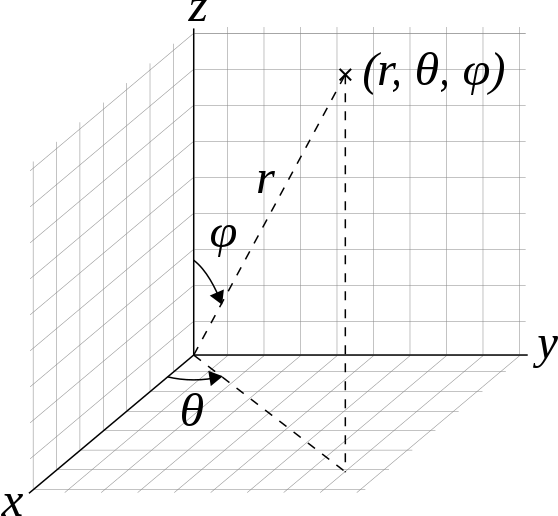
\includegraphics[width=0.7\textwidth]{figure1.png} 
\end{figure}

Given polar angle $\phi \in (0, \pi)$ and azimuthal angle $\theta \in (0, 2\pi)$, we have:

$$x = rsin(\phi)cos(\theta)$$
$$y = rsin(\phi)sin(\theta)$$
$$z = rcos(\phi)$$

Let $v$ be a point on the unit sphere $S$. We want probability density $p(v)$ to be a constant. Since $\int_S p(v) dA = 1$, we obtain:

$$p(v) = \frac{1}{4\pi}$$

We want to represent point $v$ with spherical coordinates $\theta$ and $\phi$ and find the probability density function $p(\phi, \theta)$:

$$p(v) dA = \frac{1}{4\pi} dA = p(\phi, \theta) d\phi d\theta$$

Since $dA = sin\phi d\phi d\theta$, we have:

$$p(\phi, \theta) = \frac{sin \phi}{4 \pi}$$

We can get probability density function of $\phi$ and $\theta$ respectively:

$$p(\phi) = \int_{0}^{2\pi} p(\phi, \theta) d\theta = \int_{0}^{2\pi} \frac{sin\phi}{4\pi} d\theta = \frac{sin\phi}{2}$$

$$p(\theta) = \int_{0}^{\pi} p(\phi, \theta) d\phi = \int_{0}^{\pi} \frac{sin\phi}{4\pi} d\phi = \frac{1}{2\pi}$$

We find $p(\phi)$ scales with $sin\phi$ and $\theta$ is a uniformly distributed variable.

$\\$
The algorithm for sampling the distribution $p(\phi)$ using inverse transform sampling is as follows:
\begin{itemize}
\item Generate a uniform random number $\zeta$ from the distribution $U$[0, 1]
\item Compute $\phi$ such that cumulative distribution function $F(\phi) = \zeta$, i.e. $F^{-1}(\zeta)$
\item This $\phi$ is a random number from the distribution $f(\phi)$
\end{itemize}

$\\$
Based on inverse transform sampling, we need cumulative distribution function of $\phi$
$$F(\phi) = \int_{0}^{\phi} p(\phi') d\phi' = \int_{0}^{\phi} \frac{sin\phi'}{2} d\phi' = \frac{1}{2}(1 - cos\phi)$$

We can obtain $\phi$:

$$\phi = arccos(1 - 2\zeta)$$

$\\$
The algorithm below in C++ shows how to generate uniformly distribution points on a sphere using this method:

\begin{lstlisting}
#include <chrono>
#include <random>
#include <math.h>
#include <iostream>

int main(int argc, char *argv[]){
    unsigned seed = std::chrono::system_clock::now().time_since_epoch().count();
    std::mt19937 generator(seed);
    std::uniform_real_distribution<double> uniform01(0.0, 1.0);

    int n = 10;

    for (int i = 0; i < n; ++i){
        double phi = acos(1 - 2 * uniform01(generator));
        double theta = 2 * M_PI * uniform01(generator);
        double x = sin(phi) * cos(theta);
        double y = sin(phi) * sin(theta);
        double z = cos(phi);

        std::cout << theta << ", " << phi << ", " << x << ", " << y << ", " << z <<std::endl;
    }
    
    return 0;
}
\end{lstlisting}

$\\$
According to the algorithm above, the probability density function of $\theta$ is constant, we only need to verify whether points are uniform along $\phi$ axis in spherical coordiantes. We first choose the region with $z$-coordiate $>= z$, and count the number of points in it. Then we rotate this region $\frac{\pi}{m}$ angle along $X$-axis and count the number of points in it. Repeat to rotate region and count the number. Finally we compare the numbers and plot the figure.

$\\$
Before we do the verification process, we need to figure out how to count the number of points in the rotated regions. Instead of rotating the region, we rotate the coordiantes using the following formula:

\[
\begin{bmatrix}
x_{new}\\
y_{new}\\
z_{new}\\
1
\end{bmatrix}
=
\begin{bmatrix}
1 & 0 & 0 & 0\\
0 & cos\theta & -sin\theta & 0\\
0 & sin\theta & cos\theta & 0\\
0 & 0 & 0 & 1
\end{bmatrix}
\times
\begin{bmatrix}
x_{old}\\
y_{old}\\
z_{old}\\
1
\end{bmatrix}
\]

$\\$
After getting the rotated coordiantes, we can simply count the points with $z_{new}$-coordiate $>= z$.

$\\$
Therefore our verification process is as follows:
\begin{enumerate}
\item Generate n points based on algorithm above
\item Count the number of points with $z$-coordiate $>= z$
\item Rotate the coordiate $\frac{\pi}{m} \times i$ angle along $X$-axis ($i = 0 \dots m-1$)
\item Compute the new coordiates of points after rotation
\item Repeat Step 2 to Step 4 $m$ times
\item Compare $m$ numbers
\end{enumerate}

$\\$
In order to compare our algorithm with non-uniform algorithm, we use another algorithm using:

$$\phi = \pi \times \zeta$$

$\zeta$ is a uniform random number from the distribution $U$[0, 1]

$\\$
We use $n = 100000$, $m = 20$, $z = 0.9$ and plot $m$ numbers with $i$
\begin{figure}[H]
    \centering 
    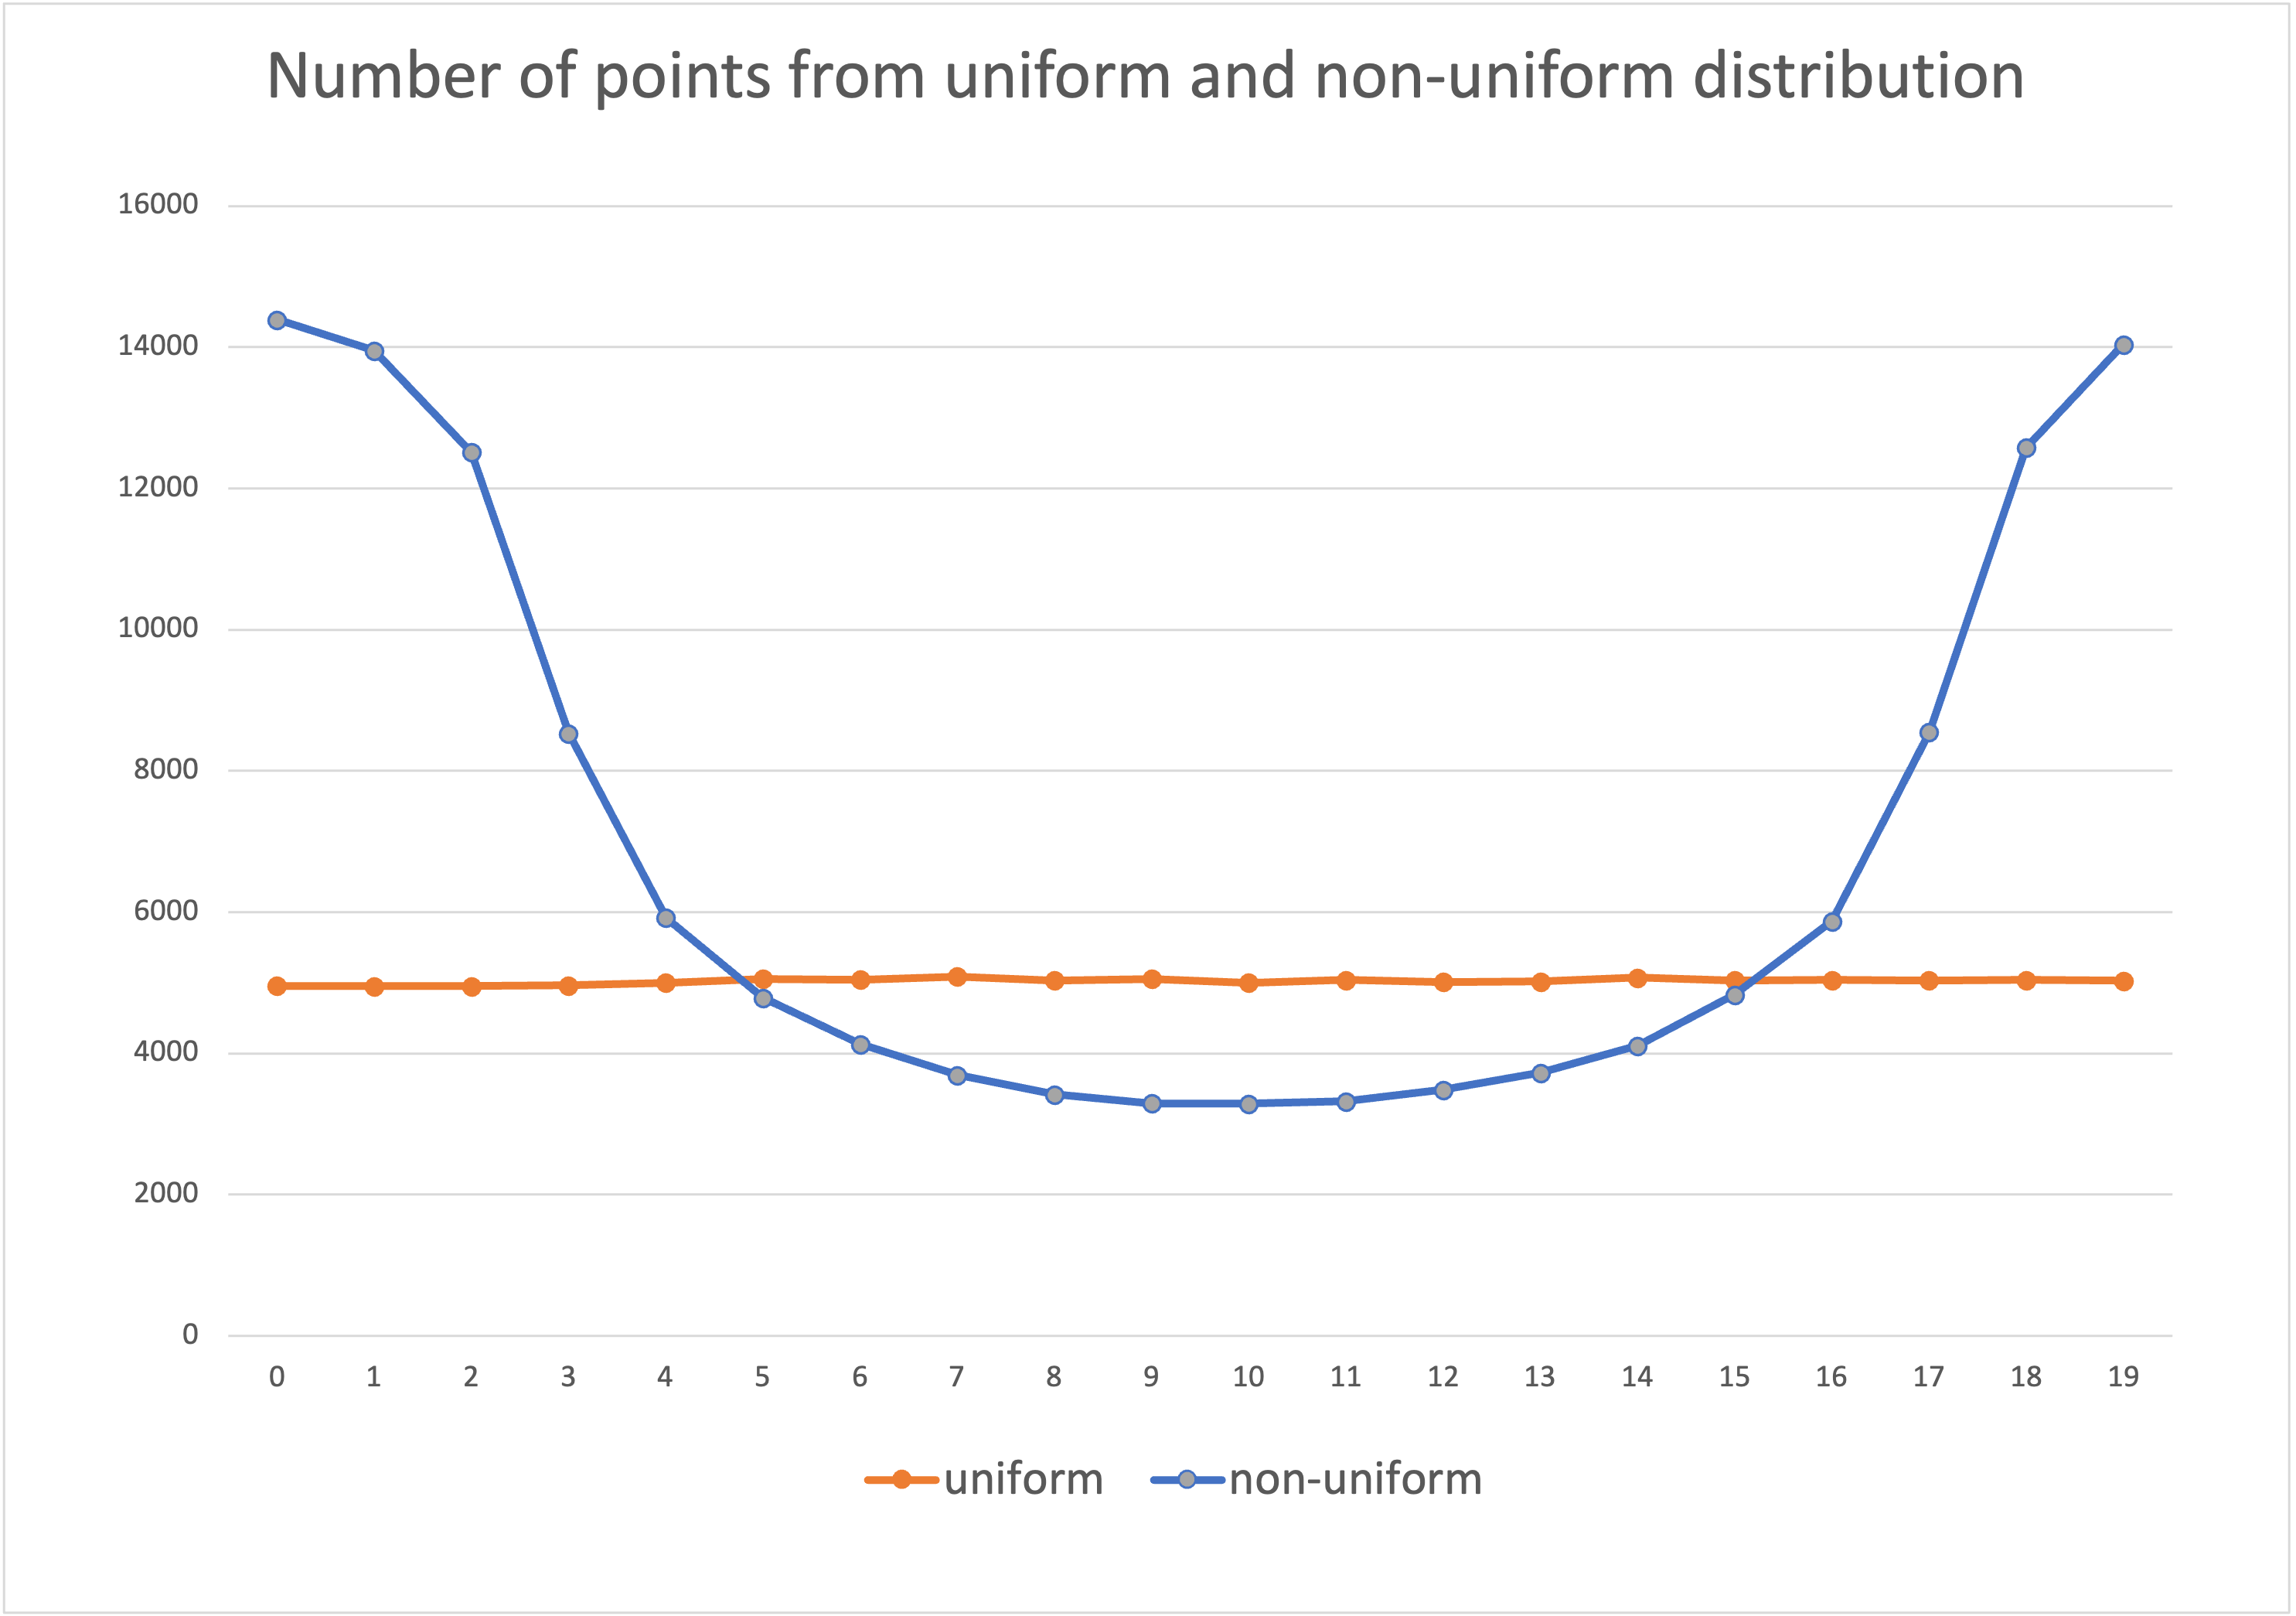
\includegraphics[width=0.7\textwidth]{figure2.png} 
\end{figure}

We find that points generated from our algorithm are relatively uniform.

$\\$
C++ code including verification is as follows.

Note: in Line 26 and 35, we can use reference to vector instead of vector itself to eliminate copy constructor, but there are bugs that latex cannot recognize reference symbol:

\begin{lstlisting}
#include <chrono>
#include <random>
#include <math.h>
#include <iostream>

std::vector<std::vector<double>> uniform_points(int num){
    double phi, theta;
    std::vector<std::vector<double>> points(num);

    unsigned seed = std::chrono::system_clock::now().time_since_epoch().count();
    std::mt19937 generator(seed);
    std::uniform_real_distribution<double> uniform01(0.0, 1.0);

    for (int i = 0; i < num; ++i){
        phi = acos(1 - 2 * uniform01(generator));
        theta = 2 * M_PI * uniform01(generator);

        points[i].push_back(sin(phi) * cos(theta));
        points[i].push_back(sin(phi) * sin(theta));
        points[i].push_back(cos(phi));
    }

    return points;
}

int count_points(std::vector<std::vector<double>> points, double z){
    int count = 0;
    for (auto point: points){
        if (point[2] >= z)
            ++count;
    }
    return count;
}

std::vector<std::vector<double>> rotate_x(std::vector<std::vector<double>> points, double theta){
    int size = points.size();
    std::vector<std::vector<double>> rotate_points(size);

    double x, y, z;

    for (int i = 0; i < size; ++i){
        x = points[i][0];
        y = points[i][1];
        z = points[i][2];

        rotate_points[i].push_back(x);
        rotate_points[i].push_back(y * cos(theta) - z * sin(theta));
        rotate_points[i].push_back(y * sin(theta) + z * cos(theta));
    }

    return rotate_points;
}

std::vector<std::vector<double>> not_uniform_points(int num){
    double phi, theta;
    std::vector<std::vector<double>> points(num);

    unsigned seed = std::chrono::system_clock::now().time_since_epoch().count();
    std::mt19937 generator(seed);
    std::uniform_real_distribution<double> uniform01(0.0, 1.0);

    for (int i = 0; i < num; ++i){
        phi = M_PI * uniform01(generator);
        theta = 2 * M_PI * uniform01(generator);

        points[i].push_back(sin(phi) * cos(theta));
        points[i].push_back(sin(phi) * sin(theta));
        points[i].push_back(cos(phi));
    }

    return points;
}

int main(int argc, char *argv[]){
    int n = 100000;
    int m = 20;
    double z = 0.9;

    std::vector<std::vector<double>> points;
    std::vector<std::vector<double>>rotate_points;

    std::cout << "uniform:" << std::endl;
    points = uniform_points(n);
    for (int i = 0; i <= m - 1; ++i){
        rotate_points = rotate_x(points, M_PI / m * i);
        std::cout << count_points(rotate_points, z) << std::endl;
    }

    std::cout << "non-uniform:" << std::endl;
    points = not_uniform_points(n);
    for (int i = 0; i <= m - 1; ++i){
        rotate_points = rotate_x(points, M_PI / m * i);
        std::cout << count_points(rotate_points, z) << std::endl;
    }

    return 0;
}
\end{lstlisting}

\end{document}